\PassOptionsToPackage{no-math,cm-default}{fontspec}
\documentclass[twoside,nofonts,internet]{askhseis}
\usepackage{amsmath}
\usepackage{xgreek}
\let\hbar\relax
\defaultfontfeatures{Mapping=tex-text,Scale=MatchLowercase}
\setmainfont[Mapping=tex-text,Numbers=Lining,Scale=1.0,BoldFont={Minion Pro Bold}]{Minion Pro}
\newfontfamily\scfont{GFS Artemisia}
\font\icon = "Webdings"
\usepackage{mtpro2}
\usepackage{multicol}
\usepackage{hhline}
\usepackage{pgfplots}
\xroma{blue!50!green}
\newcommand{\tss}[1]{\textsuperscript{#1}}
\newcommand{\tssL}[1]{\MakeLowercase\textsuperscript{#1}}
\pgfkeys{/pgfplots/aks_on/.style={axis lines=center,
xlabel style={at={(current axis.right of origin)},xshift=1.5ex, anchor=center},
ylabel style={at={(current axis.above origin)},yshift=1.5ex, anchor=center}}}
\pgfkeys{/pgfplots/grafikh parastash/.style={cyan,line width=.4mm,samples=200}}
\pgfkeys{/pgfplots/belh ar/.style={tick label style={font=\scriptsize},axis line style={-latex}}}


\begin{document}
\titlos{Μαθηματικά Α΄ Γυμνασίου}{Φυσικοί Αριθμοί}{Φυσικοί Αριθμοί - Διάταξη - Στρογγυλοποίηση}
\twocolumn
\thewria
\begin{enumerate}[itemsep=5mm]
\item \textbf{Ερωτήσεις θεωρίας}\\
Να απαντήσετε στις παρακάτω ερωτήσεις.
\begin{rlist}
\item Ποιους αριθμούς περιέχει το σύνολο των φυσικών αριθμών;
\item Από όλους τους φυσικούς αριθμούς ποιος είναι αυτός που δεν έχει προηγούμενο αριθμό;
\item Τί ονομάζουμε άξονα των φυσικών αριθμών;
\item Τι ονομάζουμε στρογγυλοποίηση;
\item Ποιες είναι οι δεκαδικές αξίες ενός επταψήφιου αριθμού;
\end{rlist}
\item \textbf{Σωστό - Λάθος}\\
Να χαρακτηρίσετε τις παρακάτω προτάσεις ως σωστές (Σ) ή λανθασμένες (Λ).
\begin{rlist}
\item Σε έναν φυσικό αριθμό η θέση των δεκάδων χιλιάδων (ΔΧ) δηλώνει μεγαλύτερη αξία πό τη θέση των χιλιάδων (Χ).
\item Στο φυσικό αριθμό $ 39.817 $ το ψηφίο $ 9 $ είναι στη θέση των δεκάδων χιλιάδων.
\item Ανάμεσα σε δύο τριψήφιους αριθμούς, μεγαλύτερος είναι εκείνος που έχει περισσότερες εκατοντάδες (Ε).
\item Ανάμεσα σε δύο φυσικούς αριθμούς, μεγαλύτερος είναι εκείνος που έχει περισσότερες εκατοντάδες (Ε).
\item Όταν στρογγυλοποιούμε έναν αριθμό τότε η αξία του αριθμού αυτού μειώνεται.
\end{rlist}
\item \textbf{Αντιστοίχηση}\\
Να αντιστοιχήσετε τις προτάσεις τις 1\tss{ης} στήλης με τις σωστές προτάσεις από τη 2 \tss{η} στήλη.
\vspace{-1.1cm}
\begin{flushleft}
\begin{tabular}{p{3.7cm}p{3.7cm}}
\begin{rlist}[leftmargin=2mm]
\item Ο αριθμός $ 3.918 $ έχει
\item Ο αριθμός $ 8.194 $ έχει
\item Ο αριθμός $ 7.823 $ έχει
\item Ο αριθμός $ 1.395 $ έχει
\item Ο αριθμός $ 9.027 $ έχει
\end{rlist} & 
\begin{rlist}
\item $ 3 $ εκατοντάδες
\item $ 2 $ δεκάδες
\item $ 9 $ χιλιάδες
\item $ 4 $ μονάδες
\item $ 3 $ χιλιάδες
\end{rlist} \\ 
\end{tabular} 
\end{flushleft}
\vspace{-.8cm}
\item \textbf{Πολλαπλής επιλογής}\\
Να επιλέξετε τη σωστή απάντηση στις παρακάτω ερωτήσεις, αιτιολογώντας την επιλογή σας.
\begin{rlist}
\item Ποιος από τους παρακάτω αριθμούς είναι μεγαλύτερος;
\begin{multicols}{4}
\begin{itemize}
\item $ 928 $
\item $ 982 $
\item $ 988 $
\item $ 908 $
\end{itemize}
\end{multicols}
\vspace{-3mm}
\item Ποιος από τους παρακάτω αριθμούς είναι μικρότερος;
\begin{multicols}{4}
\begin{itemize}
\item $ 409 $
\item $ 490 $
\item $ 410 $
\item $ 499 $
\end{itemize}
\end{multicols}
\vspace{-3mm}
\item Ποιος από τους παρακάτω αριθμούς δεν ανήκει στο σύνολο των φυσικών αριθμών;
\begin{multicols}{4}
\begin{itemize}
\item $ 7 $
\item $ 3{,}5 $
\item $ 0 $
\item $ 15 $
\end{itemize}
\end{multicols}
\item Αν στρογγυλοποιήσουμε τον αριθμό $ 15.729 $ στη δεκαδική θέση των χιλιάδων (Χ) τότε ποιος από τους παρακάτω αριθμούς προκύπτει;
\begin{multicols}{3}
\begin{itemize}
\item $ 15.000 $
\item $ 15.700 $
\item $ 16.000 $
\end{itemize}
\end{multicols}
\end{rlist}
\item \textbf{Συμπλήρωση κενών}\\
Να συμπληρώσετε τα κενά στις παρακάτω προτάσεις.
\begin{rlist}
\item Κάθε φυσικός αριθμός έχει έναν \ldots\ldots\ldots\ldots\, και έναν επόμενο αριθμό, εκτός από το 0 το οποίο έχει μόνο \ldots\ldots\ldots\ldots
\item Η διάταξη είναι η ιδιότητα των φυσικών αριθμών η οποία μας επιτρέπει να \ldots\ldots\ldots\ldots\, φυσικούς αριθμούς μεταξύ τους και τα τους τοποθετούμε σε σειρά.
\item Στη στρογγυλοποίηση ενός αριθμού αν το ψηφίο αμέσως μικρότερης αξίας από τη θέση στρογγυλοποίησης είναι ένα από τα \ldots\ldots\ldots\ldots,\, τότε το ψηφίο της θέσης στρογγυλοποίησης αυξάνεται κατά 1 ενώ όλα τα επόμενα μηδενίζονται.
\item Στη στρογγυλοποίηση ενός αριθμού αν το ψηφίο αμέσως μικρότερης αξίας από τη θέση στρογγυλοποίησης είναι ένα από τα \ldots\ldots\ldots\ldots,\, τότε το ψηφίο της θέσης στρογγυλοποίησης παραμένει ίδιο ενώ όλα τα επόμενα μηδενίζονται.
\item Για να συγκρίνουμε δύο φυσικούς αριθμούς μεταξύ τους, ξεκινάμε τον έλεγχο από το ψηφίο της \ldots\ldots\ldots\ldots\, αξίας κάθε αριθμού.
\end{rlist}
\end{enumerate}
\askhseis
\begin{enumerate}[itemsep=5mm]
\item \textbf{Φυσικοί αριθμοί}\\
Να σχηματίσετε τον αριθμό με τα ψηφία που περιέχει κάθε στήλη στον παρακάτω πίνακα, τοποθετημένα στη σωστή σειρά.
\begin{center}
\begin{tabular}{c|c|c|c|c} 
\hline \rule[-1.5ex]{0pt}{5ex} Δεκ. Θέση & 1\tss{ος} & 2\tss{ος} & 3\tss{ος} & 4\tss{ος} \\ 
\hhline{=====} \rule[-1.5ex]{0pt}{5ex} Δεκάδες & 3 & 2 & 5 & 7 \\ 
\rule[-1.5ex]{0pt}{5ex} Χιλιάδες & 4 & 8 & 3 & 0 \\ 
\rule[-1.5ex]{0pt}{5ex} Μονάδες & 8 & 7 & 3 & 2 \\ 
\rule[-1.5ex]{0pt}{5ex} Εκατοντάδες & 1 & 1 & 0 & 3 \\ 
\rule[-1.5ex]{0pt}{5ex} Δεκάδες Χιλιάδες & 0 & 6 & 4 & 9 \\ 
\hline 
\end{tabular} 
\end{center}
\item \textbf{Φυσικοί αριθμοί}\\
Να γράψετε όλους τους αριθμούς που μπορούν να σχηματιστούν χρησιμοποιώντας τα ψηφία $ 7,3,8 $.
\begin{rlist}
\item Ποιος από όλους αυτούς είναι ο μεγαλύτερος και ποιος ο μικρότερος;
\item Πόση διαφορά έχει ο μεγαλύτερος από το μικρότερο;
\end{rlist}
\item \textbf{Φυσικοί αριθμοί}\\
Γράψτε τον προηγούμενο και τους δύο επόμενους φυσικούς των παρακάτω αριθμών.
\begin{multicols}{3}
\begin{rlist}
\item $ 124 $
\item $ 592 $
\item $ 3.782 $
\item $ 4.098 $
\item $ 1.001 $
\item $ 13.999 $
\end{rlist}
\end{multicols}
\item \textbf{Φυσικοί Αριθμοί}\\
Να γράψετε όλους τους φυσικούς αριθμούς που βρίσκονται ανάμεσα από
\begin{multicols}{2}
\begin{rlist}
\item $ 173 $ και $ 187 $
\item $ 212 $ και $ 224 $
\item $ 369 $ και $ 385 $
\item $ 457 $ και $ 468 $
\item $ 798 $ και $ 803 $
\item $ 1.274 $ και $ 1.290 $
\end{rlist}
\end{multicols}
\item \textbf{Φυσικοί Αριθμοί}\\
Δίνεται ο φυσικός αριθμός $ 3.847 $. Να υπολογίσετε τον αριθμό που θα σχηματιστεί αν τον
\begin{rlist}
\item αυξήσουμε κατά $ 3 $ μονάδες, $ 4 $ δεκάδες και $ 2 $ εκατοντάδες.
\item αυξήσουμε κατά $ 9 $ μονάδες, $ 2 $ δεκάδες και $ 5 $ εκατοντάδες.
\item μειώσουμε κατά $ 8 $ μονάδες, $ 2 $ δεκάδες και $ 3 $ εκατοντάδες.
\end{rlist}
\item \textbf{Διάταξη}\\
Να συμπληρώσετε τα παρακάτω κενά με το σωστό σύμβολο ισότητας ή ανισότητας : $ =,<,> $.
\begin{multicols}{2}
\begin{rlist}
\item $ 3.478\ldots3.487 $
\item $ 289\ldots299 $
\item $ 1.398\ldots1.389 $
\item $ 10.001\ldots1.001 $
\item $ 2.020\ldots2.020 $
\item $ 4.901\ldots4.910 $
\end{rlist}
\end{multicols}
\item \textbf{Διάταξη}\\
Να τοποθετήσετε τους παρακάτω αριθμούς σε σειρά από το μικρότερο στο μεγαλύτερο.
\begin{rlist}
\item $ 3.899, 3.989,3.888,3.099,3.998,3.889 $
\item $ 2.220,2.022,2.202,2.002,2.020,2.222 $
\end{rlist}
\item \textbf{Διάταξη}\\
Να τοποθετήσετε τους παρακάτω αριθμούς σε σειρά από το μεγαλύτερο στο μικρότερο.
\begin{rlist}
\item $ 4.090,4.009,4.909,4.990,4.099,4.999 $
\item $ 7.797,7.997,7.097,7.979,7.977,7.777 $
\end{rlist} 
\item \textbf{Στρογγυλοποίηση}\\
Να στρογγυλοποιήσετε καθέναν από τους παρακάτω αριθμούς στις
\begin{multicols}{3}
\begin{itemize}[leftmargin=2mm]
\item Δεκάδες
\item Χιλιάδες
\item Εκατοντάδες
\end{itemize}
\end{multicols}
\begin{multicols}{2}
\begin{rlist}
\item $ 1.734 $
\item $ 4.567 $
\item $ 9.392 $
\item $ 2.083 $
\end{rlist}
\end{multicols}
\item \textbf{Στρογγυλοποίηση}\\
Να στρογγυλοποιήσετε τον αριθμό $ 7.394.751 $ στο ψηφίο των
\begin{multicols}{2}
\begin{rlist}
\item δεκάδων
\item εκατοντάδων
\item χιλιάδων
\item δεκ. χιλιάδων
\item εκ. χιλιάδων
\item εκατομμυρίων
\end{rlist}
\end{multicols}
\item \textbf{Άξονας των αριθμών}\\
Να κατασκευάσετε έναν άξονα φυσικών αριθμών με αρχή το σημείο $ O $ όπου κάθε μονάδα απέχει από την επόμενη $ 1\,cm $.
\begin{center}
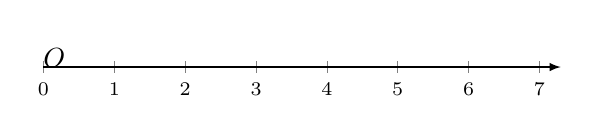
\begin{tikzpicture}
\tkzSetUpPoint[size=7,fill=white]
\clip (-.2,-.5) rectangle (6.8,0.5);
\begin{axis}[aks_on,belh ar,axis y line=none,xmin=0,xmax=7.3,x=.9cm,ymin=0,ymax=2]
\end{axis}
\tkzDrawPoint(0,0)
\tkzLabelPoint[above](0,0){$O$}
\end{tikzpicture}
\end{center}
Στη συνέχεια να πάρετε σημεία $ A,B,\varGamma $ πάνω στον άξονα ώστε $ OA=3\,cm $, $ AB=7\,cm $ και $ B\varGamma=2\,cm $. Σε ποιους αριθμούς αντιστοιχούν αυτά τα σημεία;
\item \textbf{Άξονας των αριθμών}\\
Κατασκευάσαμε τον άξονα των φυσικών αριθμών έτσι ώστε κάθε μονάδα απέχει από την επόμενη $ 1\,cm $ και τοποθετήσαμε τους αριθμούς $ 2.928 $, $ 2.930 $ και $ 2.899 $.
\begin{rlist}
\item Ποιος απ' αυτούς τους αριθμούς έχει μεγαλύτερη απόσταση από την αρχή $ O $ του άξονα και ποιος τη μικρότερη;
\item Πόση απόσταση έχει ο 1\tss{ος} αριθμός από τον 3\tss{ο} καί πόση από τον 2\tss{ο};
\end{rlist}
\item \textbf{Σύνθετη Άσκηση}\\
Σε έναν τετραψήφιο αριθμό το ψηφίο των δεκάδων είναι το ίδιο με το ψηφίο των χιλιάδων. Επίσης ο αριθμός αυτός έχει 7 εκατοντάδες ενώ το ψηφίο των μονάδων είναι κατά 2 μικρότερο από το ψηφίο των δεκάδων. Αν γράψουμε τα ψηφία του αριθμού αυτού με αντίστροφη σειρά τότε ο αριθμός που προκύπτει είναι τριψήφιος. Ποιος είναι ο αρχικός αριθμός;
\item \textbf{Πρόβλημα}\\
Σε έναν κλασικό αγώνα με βελάκια δύο παίκτες συμφωνούν να ρίξουν 10 βολές ο καθένας και στοιχηματίζουν ένα χρηματικό ποσό για το ποιος θα φέρει το μεγαλύτερο αποτέλεσμα.
\tikzstyle{wired}=[draw=gray!30, line width=0.15mm]
\tikzstyle{number}=[anchor=center, color=white]
% Sectors are numbered 0-19 counterclockwise from the top.

% \strip{color}{sector}{outer_radius}{inner_radius}
\newcommand{\strip}[4]{
	\filldraw[#1, wired]
	({18 *  #2}      :                   #3) arc
	({18 *  #2}      : {18 * (#2 + 1)} : #3) --
	({18 * (#2 + 1)} :                   #4) arc
	({18 * (#2 + 1)} : {18 *  #2}      : #4) -- cycle;
}

% \sector{color}{sector}{radius}
\newcommand{\sector}[3]{
	\filldraw[#1, wired]
	(0, 0) --
	({18 * #2} :                   #3) arc
	({18 * #2} : {18 * (#2 + 1)} : #3) -- cycle;
}


% 81 degrees = 4.5 sectors.
% The rotation leaves 20 at the top.
\begin{center}
	\begin{tikzpicture}[rotate=81, scale=.09]

% These are the official dartboard dimensions as per BDO's regulations.

% The whole board's background.
\fill[black] (0, 0) circle (225.5mm);

% Even sections.
\foreach\i in {0,2,...,18} {
	\sector{black}{\i}{162mm}
	\strip{black!40}{\i}{170mm}{162mm} % Double strip.
	\strip{black!40}{\i}{107mm}{ 99mm} % Treble strip.
}

% Odd sections.
\foreach\i in {1,3,...,19} {
	\sector{white}{\i}{162mm}
	\strip{\xrwma!80}{\i}{170mm}{162mm} % Double strip.
	\strip{\xrwma!80}{\i}{107mm}{ 99mm} % Treble strip.
}

% Bull's ring and eye.
\filldraw[\xrwma!50, wired] (0, 0) circle (15.9mm);
\filldraw[black,   wired] (0, 0) circle (6.35mm);

% Labels.
\foreach \sector/\label in {%
	0/20,  1/ 1,  2/18,  3/ 4,  4/13,
	5/ 6,  6/10,  7/15,  8/ 2,  9/17,
	10/ 3, 11/19, 12/ 7, 13/16, 14/ 8,
	15/11, 16/14, 17/ 9, 18/12, 19/ 5}
{
	\node[number] at ({18 * (-\sector + .5)} : 197.75mm) {\label};
}
\end{tikzpicture}
\end{center}
Το σκορ του παίκτη Α μέχρι και την ένατη βολή είναι $ 139 $ μονάδες ενώ ο παίκτης Β στις 9 βολές έχει συγκεντρώσει $ 147 $ μονάδες. Στη 10\tss{η} βολή ο παίκτης Α πετυχαίνει τον αριθμό $ 17 $.
\begin{rlist}
\item Ποιόν αριθμό πρέπει να πετύχει ο παίκτης Β ώστε το σκορ του να είναι
\begin{itemize}
\item $10$ μονάδες περισσότερο
\item $4$ μονάδες λιγότερο
\end{itemize}
από το σκορ του παίκτη Α;
\item Ποιος είναι ο μεγαλύτερος αριθμός που μπορεί πετύχει ο παίκτης Β ώστε να κερδίζει το παιχνίδι ο παίκτης Α;
\item Πόσες μονάδες χρειάζεται ο παίκτης Β για να κερδίσει;
\end{rlist}
\end{enumerate}%12,14 leipoun apoth bash
\end{document}